\chapter{تخصیص منابع در شبکه های \lr{Open RAN}}
\section{مقدمه}
در این فصل، هدف تخصیص منابع در شبکه های \lr{Open RAN} در لینک فروسو می باشد که شامل تخصیص توان و برش های شبکه است.
در این بخش فرض بر این است که در شبکه ی نسل پنجم مخابرات از زیرساخت \lr{Open RAN} استفاده شده است. این شبکه سرویس هایی از قبیل \lr{IoT}، سرویس تلفن، پیامک و ... در اختیار کاربران قرار می دهد. در اینجا  مفهوم برش شبکه در سیستم بدین صورت به کار رفته که به جای دیدن کاربران به صورت مجزا، کاربرانی که از یک سرویس خاص استفاده می نمایند در دسته ی آن سرویس قرار گرفته و دسته بندی می شوند. همچنین برش هایی از شبکه در اختیار کاربران هر سرویس خاص، قرار می گیرد که هر برش شبکه شامل تعدادی واحد رادیویی
\LTRfootnote{Radio Unit}
(\lr{RU}) 
،
بلوک های منبع فیزیکی
 \LTRfootnote{Physical Resource Block}
 (\lr{PRB})، 
 یک واحد توزیع شده
\LTRfootnote{Distributed Unit}
(\lr{DU}) 
 ، 
 یک واحد مرکزی
\LTRfootnote{Centralized Unit}
(\lr{CU})  
  می باشد که هر واحد توزیع شده و مرکزی شامل تعدادی توابع شبکه ی مجازی شده
  \LTRfootnote{Virtual Network Function}
(\lr{VNF}) 
می باشد. 

در این سیستم هدف، بررسی مسئله ی برش شبکه در بخش RAN و بخشی از هسته در شبکه های دسترسی باز
ORAN
می باشد.
ما مسئله زمانبندی لینک بی سیم، اختصاص برشها به سرویسها و اختصاص مراکز داده به برشها را که از مشکلات بسته بندی جعبه  ۳-بعدی است را فرموله می کنیم. 
هدف این است که به طور مشترک بهره وری انرژی را به حداکثر برسانیم و مصرف توان واحدهای رادیویی را کاهش داده تا هزینه منابع فیزیکی را در یک کانال فروسو به حداقل برسانیم.
این مسئله به صورت یک مسئله ی 
mixed-integer
بیان می شود و به دو مسئله ی کوچکتر قابل جداسازی است. با استفاده از الگوریتمهای ابتکاری، این مسائل حل شده اند.
\begin{figure}
	\centering
	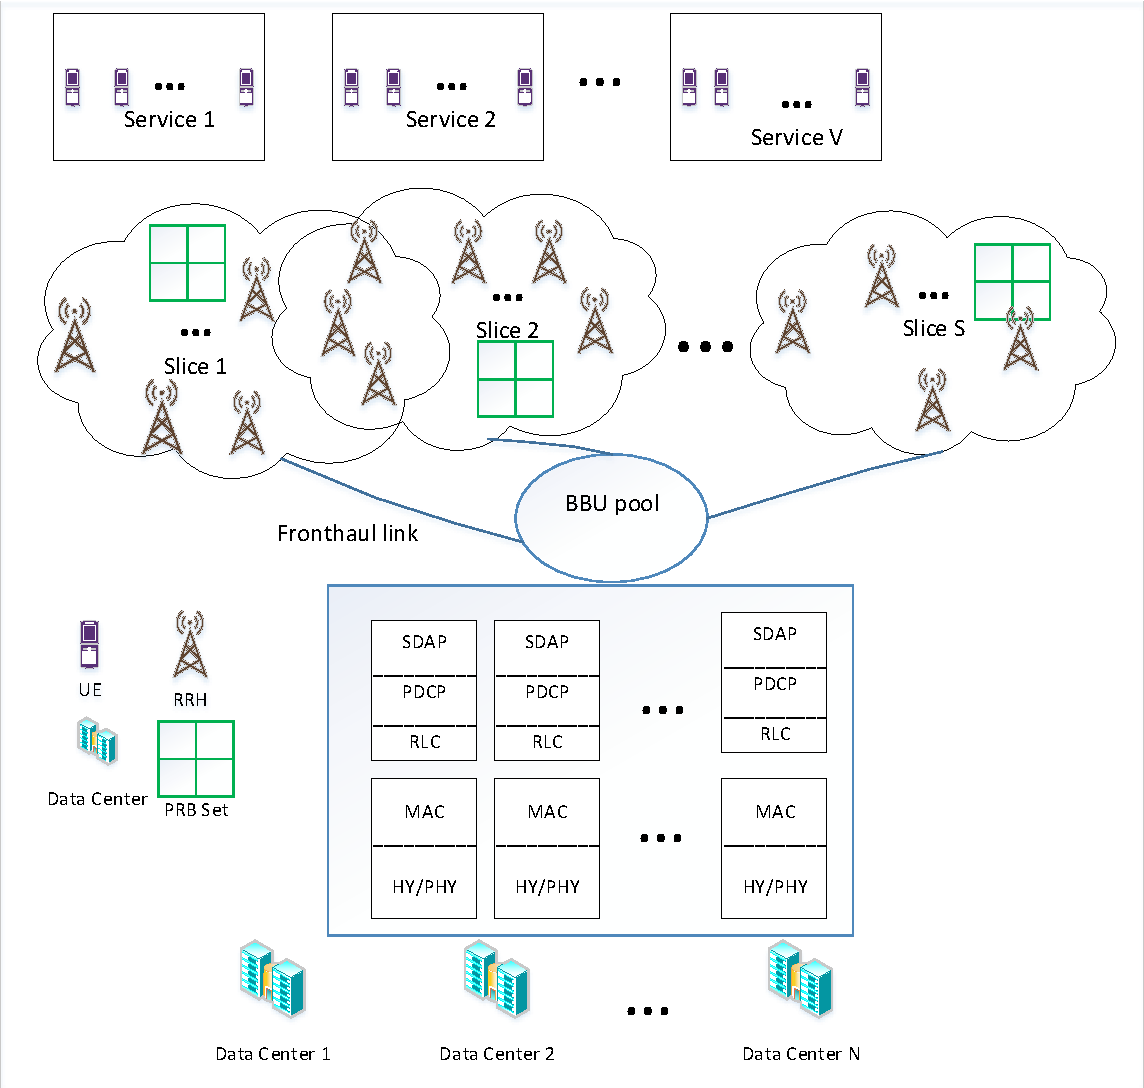
\includegraphics[scale=0.55]{./fig/c2.pdf}
	\caption{برش شبکه در ORAN}
	\label{fig:c11}
\end{figure}
در شکل \ref{fig:c11}
لینک فروسو در سیستم ORAN نشان داده شده است که بخش RAN به سه لایه تقسیم می‌گردد که شامل بخش RU، 
CU و
بخش DU می‌باشد.
بخش CUو DU برروی مرکز داده اجرا می‌شوند. کاربران براساس نیاز سرویسهای مختلف تقسیم شده‌اند.

نوآوری های این کار در ادامه بیان شده است.
\begin{itemize}
\item 
به طور همزمان برش شبکه و تخصیص منابع در سیستم
 ORAN
  در نظر گرفته شده است.
\item 
مسئله ی پذیرش کاربر و تخصیص خدمات به برش ها، و منابع فیزیکی بی سیم و مرکز داده به برش ها را به عنوان یک مسئله ی بهینه سازی حل می کنیم.
\item
از الگوریتمهای ابتکاری در جهت حل این مسائل برای رسیدن به پاسخ نسبتا بهینه استفاده کرده تا در کمترین زمان پاسخ نسبتا بهینه را بدهد.
\end{itemize} 
\section{مدل سیستم}
در این قسمت، سیستم مدل به صورت کامل مورد بررسی قرار می گیرد.
فرض می کنیم $S$ برش شبکه داریم که قرار است $V$ سرویس مختلف که شامل کاربرانی است که از سرویس خاص استفاده می نمایند را سرویس دهی نماید.
هر سرویس 
$v\in \{1,2,...,V \} $
شامل 
$U_v$
کاربر تک آنتنه می باشند که سرویس خاصی را درخواست می نماید.
هر برش شبکه 
$s \in \{1,2,...,S \}$
شامل 
$R_s$
واحد رادیویی،
$K_s$
بلوک های منابع فیزیکی، یک واحد توزیع شده و یک واحد مرکزی که شامل \lr{VNF} هایی می باشند.
همچنین برش های شبکه می توانند منابع مشترک داشته باشند.
تمام \lr{RU}هایی که به یک سرویس خاص خدمت رسانی می کنند به صورت مشارکتی سیگنال به تمام کاربران در آن سرویس ارسال می نمایند. 
\cite{motalleb2017optimal,mimoCran}
هر واحد رادیویی
$r \in \{1,2,...,R \}$
به یک واحد توزیع شده از طریق لینک فیبر نوری با ظرفیت \lr{fronthaul} 
محدود متصل می باشد.
در سیستم \lr{Open RAN}
دو لایه ی پردازشی که اولی در \lr{CU} و دومی در \lr{DU} قرار گرفته است که پردازش ها با \lr{VNF} ها صورت می گیرد.
لایه پایین تر (\lr{DU}) شامل 
\lr{high-PHY}
،
\lr{MAC}
و 
\lr{RLC}
می باشد و 
لایه ی بالاتر 
(\lr{CU})
شامل 
\lr{RRC}
،
\lr{PDCP}
و 
\lr{SDAP}
است.
فرض بر این است که $M_1$
\lr{VNF}
در \lr{DU}
و 
$M_2$
\lr{VNF}
در \lr{CU} قرار دارد.
هر \lr{VNF} به یک برش یا بیشتر تعلق دارد.
در $s^{th}$ امین برش شبکه $M_{s,1}$ 
\lr{VNF}
در \lr{DU}
و 
$M_{s,2}$
\lr{VNF}
دپر لایه ی \lr{CU} می باشد.
\lr{VNF}
های موجود در لایه ی \lr{DU} و \lr{VU} به ترتیب دارای ظرفیت محاسباتی 
$\mu_1$ 
و
 $\mu_2$
می باشند.
\subsection{نرخ قابل دسترس}
نرخ قابل دسترس برای $i^{th}$ امین کاربر در $v^{th}$امین سرویس به صورت زیر نوشته می شود
\begin{equation}\label{eq1}
\mathcal{R}_{u(v,i)} = B \log_2({1+ \rho_{u(v,i)}}),
\end{equation}
  که $B$ پهنای باند سیستم و 
  $\rho_{u(v,i)}$
  نسبت سیگنال به نویز $i^{th}$
  $i^{th}$ 
  امین کاربر در
   $v^{th}$
   امین سرویس
  می باشد 
  که از رابطه ی زیر بدست می آید
 \begin{equation}\label{eq2}
\rho_{u(v,i)} =  \frac{p_{u(v,i)}\sum_{s=1}^{S}|\bold{h}_{R_s,u(v,i)}^H \bold{w}_{R_s,u(v,i)}|^2 a_{v,s}}{BN_0 + I_{u(v,i)}},
\end{equation}
که   $p_{u(v,i)}$
نشان دهنده ی توان ارسالی توسط \lr{RU} به 
$i^{th}$ 
  امین کاربر در
   $v^{th}$
   امین سرویس
   است و 
 $\bold{h}_{R_s,u(v,i)} \in \mathbb{C}^{{R}_s}$
 بردار کانال گین لینک وایرلس از \lr{RU} ها در 
$s^{th}$
امین برش شبکه می باشد.
 همچنین 
$\bold{w}_{R_s,u(v,i)} \in \mathbb{C}^{{R}_s}$
نشان دهنده ی بردار بیم فرمینگ ارسالی برای \lr{RU}ها در $s$ امین برش شبکه به کاربر $i$ ام در سرویس $v$ ام می باشد.
   به علاوه، $BN_0$
   نشان دهنده ی توان نویز اضافه شونده ی گوسی می باشد و $I_{u(v,i)}$
   توان سیگنال تداخلی است.
همچنین $a_{v,s} \in \{0,1\}$
متغیر باینری است که نشان دهنده ی این است که برش شبکه ی $s$ به سرویس $v$ خدمات رسانی می کند یا نه.
درصورتی که 
 $a_{v,s} =1$
 برش شبکه ی $s$ به سرویس $v$ خدمات رسانی می کند. در غیر این صورت خدمت رسانی نمی کند.
\newline
برای بدست آوردن \lr{SNR} در فرمول \eqref{eq2}، 
فرض می شود که 
 $\bold{y}_{U_v}\in \mathbb{C}^{U_v} $
 بردار سیگنال دریافتی از همه ی کاربران در سرویس $v$ می باشد 
\begin{equation}\label{eq3}
\textstyle \bold{y}_{U_v} = \sum_{s = 1}^{S}\sum_{k=1}^{K_s} \boldsymbol{H}^H_{\mathcal{R}_s,\mathcal{U}_v} \
\mathfrak{y}_{R_s}\zeta_{U_v,k,s} a_{v,s}+ \boldsymbol{z}_{\mathcal{U}_v},
\end{equation}
که $\mathfrak{y}_{R_s} = \boldsymbol{W}_{\mathcal{R}_s,\mathcal{U}_v}\boldsymbol{P}_{U_v}^{\frac{1}{2}}\boldsymbol{x}_{\mathcal{U}_v}+ \boldsymbol{q}_{\mathcal{R}_s}$
و 
$\boldsymbol{x}_{ \mathcal{U}_v} = [x_{ u_{(v,1)}},...,x_{ u_{(v,\mathcal{U}_v)}}]^T \in \mathbb{C}^{{R}_s } $
نشان دهنده ی بردار سمبل ارسالی کاربران سرویس $v$ می باشد.
$\boldsymbol{z}_{U_v}$
نویز گوشی جمع شونده است و
$\boldsymbol{z_{U_v}} \backsim \mathcal{N}(0,N_0\boldsymbol{I}_{{U}_v})$
.
همچنین
$N_0$
توان نویز می باشد.
علاوه بر این
$\boldsymbol{q}_{R_s} \in \mathbb{C}^{{R}_s }  $
نشان دهنده ی نویز کوانتیزاسیون می باشد که از فشرده سازی سیگنال  در واحد توزیع شده بدست آمده است.
$\boldsymbol{P}_{U_v} = \diag{(p_{u_{(v,1)}}, ..., p_{u_{(v,\mathcal{U}_v)}})}$.
همچنین در اینجا، 
$\zeta_{k,s}^{U_v} \delequal \{\zeta_{k,s}^{u(v,1)},\zeta_{k,s}^{u(v,2)},...,\zeta_{k,s}^{u(v,N_{U_v})}\}$
و 
$\zeta_{k,s}^{u(v,i)} \in \{0,1\}$
پارامتر باینری می باشد که نشان دهنده ی این است که $i$ امین کابر در $v$امین سرویس امکان ارسال سیگنال خود را از طریق 
\lr{PRB}
$k$
ام دارد یا نه، در ضمن این \lr{PRB} 
 متعلق به برش $s$ ام می باشد و یا نه.
 $\boldsymbol{H}_{\mathcal{R}_s,\mathcal{U}_v}=\left[\boldsymbol{h}_{\mathcal{R}_s,u_{(v,1)}},\ldots,\boldsymbol{h}_{\mathcal{R}_s,v_{(v,\mathcal{U}_v)}}\right]^T  \in \mathbb{C}^{{R}_s\times {U}_v }$
نشان دهنده ی ماتریس کانال بین دسته واحد رادیویی 
 $\mathcal{R}_s$
 به دسته 
 $\mathcal{U}_v$
 کاربران می باشد.
بردار کانال بین $s$امین برش و $i$امین کابر در $v$امین سرویس $\boldsymbol{h}_{\mathcal{R}_s,u_{(v,i)}}\in \mathbb{C}^{{R}_s}$ به صورت زیر نشان داده شده است 
\begin{equation}
\boldsymbol{h}_{\mathcal{R}_s,u_{(s,i)}} = \boldsymbol{\beta}^\frac{1}{2}_{\mathcal{R}_s,u_{(v,i)}} \boldsymbol{g}_{\mathcal{R}_s,u_{(v,i)}},
\end{equation} 
که در اینجا 
$\boldsymbol{g}_{\mathcal{R}_s,u_{(v,i)}} \backsim \mathcal{N}(0,N_0\boldsymbol{I}_{\mathcal{U}_v})$
نشان دهنده ی بردار کانال فیدینگ سریع و تخت می باشد و
 $\boldsymbol{\beta}_{\mathcal{R}_s,u_{(v,i)}}=\text{diag}(b_{r_{(s,1),u_{(v,i)}}},\ldots,b_{r_{(s,\mathcal{R}_s),u_{(v,i)}}})$
 نشان دهنده ی ماتریس فیدینگ مقیاس بزرگ می باشد.
در اینجا فرض بر این است که اطلاعات حالت کانال \lr{CSI}، به صورت کامل می باشد.\newline
 $\boldsymbol{W}_{\mathcal{R}_s,\mathcal{U}_v} = [\boldsymbol{w}_{\mathcal{R}_s,u(v,1)},...,\boldsymbol{w}_{\mathcal{R}_s,u(v,U_v)}] \in \mathbb{C}^{{R}_s\times U_v} $
 بردار بیم فرمینگ \lr{zero forcing}
  می باشد که برای مینیمم کردن تداخل می باشد و بدین صورت است
\begin{equation}
\textstyle \boldsymbol{W}_{\mathcal{R}_s,\mathcal{U}_v} = \boldsymbol{H}_{\mathcal{R}_s,\mathcal{U}_v}(\boldsymbol{H}_{\mathcal{R}_s,\mathcal{U}_v}^H \boldsymbol{H}_{\mathcal{R}_s,\mathcal{U}_v})^{-1}.
\end{equation}  
توان تداخلی کابر $i$ام به سرویس $v$ام به صورت زیر بیان می شود
\begin{equation}
\begin{split}
 I_{u_{(v,i)}} &=
 \underbrace{\sum_{s=1}^{S}\sum_{n=1}^{S}\sum_{\substack{l=1 \\ l\neq i}}^{{U}_v} \gamma_{1}  p_{u_{(v,l)}}a_{v,s}\zeta_{u_(v,i),n,s}\zeta_{u_(v,l),n,s}}_{\text{(intra-service interference)}}\\
&+ \underbrace{\sum_{\substack{y=1 \\ l\neq v}}^{V}\sum_{s=1}^{S}\sum_{n=1}^{S}\sum_{l=1}^{{U}_y} \gamma_{2}  p_{u_{(y,l)}}a_{y,s} \zeta_{u_(v,i),n,s}\zeta_{u_(y,l),n,s}}_{\text{(inter-service interference)}}\\
&+\underbrace{ \sum_{s=1}^{S} \sum_{j=1}^{{R}_s} {\sigma_q}_{r_{(s,j)}}^2 |\boldsymbol{h}_{r_{(s,j)}, u_{(v,i)}}|^2 a_{v,s}}_{\text{(quantization noise interference)}},
\end{split}
\end{equation}
که 
$\gamma_{1} =|\boldsymbol{h}_{\mathcal{R}_s, u_{(v,i)}}^H \boldsymbol{w}_{\mathcal{R}_{s},u_{(v,l)}}|^2$
و 
$\gamma_{2} =|\boldsymbol{h}_{\mathcal{R}_s, u_{(v,i)}}^H \boldsymbol{w}_{\mathcal{R}_{s},u_{(y,l)}}|^2$.
همچنین 

${\sigma_q}_{r_{(s,j)}}$
واریانس نویز کوانتیزاسیون
$j$
امین 
واحد رادیویی در برش $s$ می باشد.
سیگنال تداخلی برای هر کاربر از سیگنالهای کاربرانی بدست می آید که از \lr{PRB} مشترکی استفاده نموده اند.
درصورت قرار دادن $P_{max}$
به جای 
$p_{u_{(v,l)}}$
و 
$p_{u_{(y,l)}}$
باند بالایی  
$\bar{I}_{u_{(v,i)}}$
برای 
$I_{u_{(v,i)}}$
بدست می آید
بنابراین،
$\bar{\mathcal{R}}_{u_{(v,i)}} \forall v , \forall i$ 
از قرار گرفتن 
$\bar{I}_{u_{(v,i)}}$
به جای 
$I_{u_{(v,i)}}$
در رابطه ی 
\eqref{eq1} و \eqref{eq2}
بدست می آید.
\newline
فرض کنید $\bar{p}_{r_{(s,j)}}$
نشان دهنده ی سیگنال ارسالی از $j$ امین واحد رادیویی در $s$ امین برش می باشد.
از رابطه ی \eqref{eq3} داریم
\begin{equation}
\bar{p}_{r_{(s,j)}} = \sum_{v=1}^{V}\boldsymbol{w}_{r_{(s,j)},\mathcal{U}_{v}} \boldsymbol{P}_{\mathcal{U}_v}^{\frac{1}{2}} \boldsymbol{P}_{\mathcal{U}_v}^{H \frac{1}{2}}   \boldsymbol{w}_{r_{(s,j)},\mathcal{U}_{v}}^H a_{v,s} + \sigma_{q_{r(s,j)}}^2.
\end{equation}
در این صورت نرخ کاربران در لینک \lr{fronthaul} بین $j$امین واحد رادیویی در برش $s$ام با واحد توزیع شده ی موجود در این برش، بدین صورت می باشد  \cite{simeone2016cloud, 1111}
\begin{equation}
C_{R_{(s,j)}} = \log{(1+\sum_{v=1}^{V}\frac{w_{r_{(s,j)},\mathcal{D}_{s}} \boldsymbol{P}_{\mathcal{U}_v}^{\frac{1}{2}} \boldsymbol{P}_{\mathcal{U}_v}^{H \frac{1}{2}}   w_{r_{(s,j)},\mathcal{U}_{v}}^H a_{v,s}}{ \sigma_{q_{r(s,j)}}^2})},
\end{equation}
که در اینجا 
$a_{v,s}$
متغیر باینری است که نشان دهنده ی این است که برش $s$ام به سرویس $v$ خدمات رسانی می کند یا نه.
\subsection{میانگین تاخیر}
فرض کنید ورود بسته های کاربران، فرآیند پوآسون با نرخ ورود 
$\lambda_{u(v,i)}$
برای $i$امین کاربر در سرویس $v$ ام می باشد.
بنابراین، در لایه ی واحد مرکزی (\lr{CU})، میانگین نرخ ورود داده ی کاربری که از خدمات برش $s$ استفاده می نماید 
$\alpha_{s_1} = \sum_{v=1}^{V}\sum_{u=2}^{U_v}a_{v,s}\lambda_{u(v,i)}$
می باشد. 
همچنین، میانگین نرخ داده ی ورودی در لایه ی \lr{DU}، تقریبا مساوی میانگین نرخ داده ی ورودی لایه ی اول 
$\alpha_{s} =\alpha_{s_1} \approx \alpha_{s_2}$
می باشد.
میانگین نرخ داده ی ورودی در لایه ی \lr{DU}، تقریبا برابر میانگین نرخ داده ی ورودی در لایه ی \lr{CU} می باشد $\alpha_{s} =\alpha_{s_1} \approx \alpha_{s_2}$.
در اینجا فرض بر این است کهدر هر لایه متعادل کننده ی ترافیک موجود است که ترافیک ورودی را به طور مساوی بین \lr{VNF} ها تقسیم می نماید\cite{frdl,luong2018novel,luong2018novel1}.
فرض کنید پردازش باند پایه هر \lr{VNF}، بوسیله ی پردازش صف \lr{M/M/1} نشان داده می شود.
هر بسته بوسیله ی یکی از \lr{VNF}های برش شبکه، پردازش می شود.
بنابراین، میانگین تاخیر برش $s$ در لایه ی اول و دوم با استفاده از مدل \lr{M/M.1} به این صورت نشان داده می شود
\begin{equation}
\begin{split}
d_{s_1} &= \frac{1}{\mu_1 - \alpha_{s}/{M_{s,1}}},\\
d_{s_2} &= \frac{1}{\mu_2 - \alpha_{s}/{M_{s,2}}}.
\end{split}
\end{equation}
در اینجا
$1/\mu_1$ و $1/\mu_2$
میانگین زمان سرویس دهی در لایه ی اول و دوم به ترتیب می باشند.
$\alpha_{s}$
نرخ ورودی است که توسط متعادل کننده ی ترافیک به طور مساوی بین \lr{VNF} ها تقسیم می شود.
نرخ ورودی هر \lr{VNF} در هر لایه از برش \lr{s}، $\alpha_{s}/{M_{s,i}}$ $ i \in \{1,2\}$ می باشد.
$d_{s_{tr}}$
تاخیر ارسال برای برش $s$ در لینک وایرلس می باشد.
نرخ داده ی ورودی لینک وایرلس برابر نرخ داده ی ورودی متعادل کننده ی ترافیک برای هر برش است
\cite{frdl}.
همچنین زمان سرویس برای صف ارسال در هر برش $s$ دارای توزیع نمایی با میانگین $1/(R_{{tot}_s})$
است و می توان به صورت صف \lr{M/M/1} مدل کرد  
\cite{frdl,luong2018novel,luong2018novel1,guo2016exploiting}.
بنابراین میانگین تاخیر لایه ی ارسال بدین صورت است
\begin{equation}
 d_{s_{tr}} = \frac{1}{R_{{tot}_s} - \alpha_{s}};
\end{equation}
 $R_{{tot}_s} =  \sum_{v=1}^{V}\sum_{u=2}^{U_v}a_{v,s}R_{u(v,i)}$ 
 کل نرخ قابل دسترس در هر برش می باشد که به سرویس خاص، تخصیص داده است.
میانگین تاخیر در هر برش نیز بدین صورت است
\begin{equation}
D_{s} = d_{s_1} + d_{s_2} + d_{s_{tr}} \forall s.
\end{equation}
\subsection{مرکز داده ی فیزیکی}
هر \lr{VNF}
نیازمند منابع فیزیکی است که شامل حافظه، نگهدارنده و پردازشگر می باشد.
فرض کنید منابع مورد نیاز برای $f$ امین \lr{VNF} در برش $s$ ام به صورت زیر می باشد
 \begin{equation}
\bar{\Omega}_{s}^f = \{\Omega_{M,{s}}^f, \Omega_{S,{s}}^f, \Omega_{C,{s}}^f \},
\end{equation}
که در اینجا 
 $\bar{\Omega}_{s}^f\in \mathbb{C}^{3}$
 و
$\Omega_{M,{s}}^f, \Omega_{S,{s}}^f, \Omega_{C,{s}}^f$
به ترتیب نشان دهنده ی مقدار حافظه، نگهدارنده و پردازشگر می باشد.
همچنین مقدار کل حافظه، نگهدارنده و پردازشگر برای همه \lr{VNF} ها در یک برش به این صورت تعریف می شود
\begin{equation}
\textstyle \bar{\Omega}_{\mathfrak{z},s}^{tot} = \sum_{f=1}^{M_{s_1} + M_{s_2}}\bar{\Omega}_{\mathfrak{z},s}^f \;\; \mathfrak{z} \in \{M, S, C\}.
\end{equation}
همچنین $D_c$ مرکز داده برای سرویس دهی به \lr{VNF} ها می باشد. هر مرکز داده شامل تعدادی سرور برای سرویس دهی است.
مقدار حافظه، نگهدارنده و پردازشگر به ترتیب با 
$\tau_{M_{j}}, \tau_{S_{j}}$
و
$\tau_{C_{j}} $
برای 
$j^{th}$
امین مرکز داده به ترتیب زیر می باشد.
\begin{equation*}
\tau_j = \{\tau_{M_{j}}, \tau_{S_{j}}, \tau_{C_{j}} \},
\end{equation*}
در این مدل سیستم، 
تخصیص منابع فیزیکی به \lr{VNF} ها در نظر گرفته شده است. 
در اینجا فرض بر این است که $y_{s,d}$ متغیر صفر و یکی است که نشان میدهد مرکز داده ی $d$ ام به $s$ امین برش متصل است یا نه.
\subsection{صورت مساله}
یک معیار مهم برای سنجش بهینگی یک سیستم ، بهره وری انرژی است که نسبت نرخ کل به توان کل می باشد.
\begin{equation}
\textstyle \eta(\boldsymbol{P},\boldsymbol{A}) := \frac{\sum\limits_{v=1}^{V} \sum\limits_{k=1}^{{U}_v}\mathcal{R}_{u_{(v,k)}} }{\sum\limits_{s=1}^{S} \sum\limits_{i=1}^{{R}_s}\bar{p}_{r_{(s,i)}}} = \frac{\mathfrak{R}_{tot}(\boldsymbol{P},\boldsymbol{A})}{P_r^{{tot}}(\boldsymbol{P},\boldsymbol{A})},
\end{equation}
که در اینجا، 
 $P_r^{tot}(\boldsymbol{P},\boldsymbol{A}) = \sum\limits_{s=1}^{S}\sum\limits_{i=1}^{{R}_s}\bar{p}_{r_{(s,i)}}$
 توان کل مصرفی تمام واحد های رادیویی در یک برشمی باشد.
همچنین 
 $\mathfrak{R}_{tot}(\boldsymbol{P},\boldsymbol{A}) = \sum\limits_{v=1}^{V} \sum\limits_{k=1}^{{U}_v}\mathcal{R}_{u_{(v,k)}} $
 نرخ تمام کاربران مصرفی تمام سرویس ها می باشد.
فرض کنید توان مصرفی پردازش باند پایه در هر مرکز داده ی $d$ که به \lr{VNF} های یک برش $s$ متصل می باشد با   
$\phi_{s,d}$
نشان داده شده است.
بنابراین می توان توان کل سیستم را برای کلیه مرکز داده های فعال که به برش متصل هستند ،بدین صورت نشان داد
\begin{equation*}
\textstyle \phi_{tot} = \sum_{s=1}^{S}\sum_{d=1}^{D_c}y_{s,d}\phi_{s,d}.
\end{equation*}
همچنین ، یک تابع هزینه برای قرار دادن \lr{VNF} ها در مرکز داده ها بدین عنوان تعریف شده است
\begin{equation}\label{eqpsi}
\textstyle  \psi_{tot} = \phi_{tot} - \nu \sum_{d=1}^{D_c}\sum_{v=1}^{V}y_{s,d}a_{v,s}
\end{equation}
که $\nu$
متغیر طراحی برای ارزش بین اولین ترم 
\eqref{eqpsi}
 است که عبارت است از کل مصرف انرژی منابع فیزیکی و ترم دوم که مقدار برش های پذیرفته شده برای داشتن منابع فیزیکی نشان داده شده است.
هدف ما این است که مجموع نرخ را به حداکثر رسانده و توان حاصل از کل (حداکثر توان تمام واحد های رادیویی و کل مصرف انرژی پردازش باند پایه را در کلیه مرکز داده ها) به طور همزمان و با وجود محدودیت هایی که به شرح زیر نوشته شده است ، به حداکثر برساند.
\begin{subequations}
\begin{alignat}{4}
\max\limits_{\boldsymbol{P}, \boldsymbol{A}, \boldsymbol{Y} }   \quad &  \eta(\boldsymbol{P},\boldsymbol{A})+ \varphi \frac{1}{\psi_{tot}(\boldsymbol{Y})} \\
\text{subject to} \quad  & \bar{p}_{r_{(s,i)}} \leq P_{max} \quad \forall s, \forall i,
 \label{c11} \\
&p_{u_{(v,k)}}  \geq 0  \quad \forall v, \forall k,\label{c12} \\
&\mathcal{R}_{u_{(v,k)}} \geq  \mathcal{R}_{u_{(v,k)}}^{min} \quad \forall v, \forall k,\label{c13} \\
&C_{r_{(s,i)}} \leq C_{r_{(s,i)}}^{max} \quad \forall s, \forall i, \label{c14}\\
&D_{s} \leq D_{s}^{max} \quad \forall s,\label{c15} \\
& \textstyle  \sum_{s=1}^{S}a_{v,s} \geq 1 \quad \forall s, \label{c21} \\
& \textstyle  \sum_{d=1}^{D_c}\sum_{v=1}^{V}y_{s,d}a_{v,s} \geq 1\times\sum_{v=1}^{V}a_{v,s} \forall s,\label{c23} \\
 &\textstyle \sum_{s=1}^{S} y_{s,d} \bar{\Omega}_{\mathfrak{z},s}^{tot}  \leq   \tau_{\mathfrak{z}_d}  \forall d, \forall \mathfrak{z}\in \mathcal{E}; \label{c22}
\end{alignat}
\label{constraints}
\end{subequations}
در اینجا،
$\boldsymbol{P} =[p_{u(v,k)}] \:\: \forall v , \forall k $
ماتریس توان برای کاربران است،
$\boldsymbol{A} =[a_{v,s}] \:\: \forall v , \forall s $
نشان دهنده ی
متغیر باینری برای اتصال برشها به سرویسها و
$\boldsymbol{Y} =[y_{s,d}]  \:\: \forall s ,  \forall d $
متغیر باینری برای اتصال
مرکز داده ی فیزیکی به VNFها می باشد.
همچنین
$\varphi$ 
متغیر وزنی برای ارزش گزاری بین ترم اول و دوم تابع هدف است.
\eqref{c11}
و
\eqref{c12}
به ترتیب
نشان دهنده ی این است که توان واحد رادیویی از حدی بیشتر نشده و توان هر کاربر یک عدد صحیح مثبت است.
علاوه براین
\eqref{c13}
منجر به افزایش نرخ هرکاربر از حد مورد نیاز می باشد.
 \eqref{c14}
  و 
  \eqref{c15}
  به ترتیب
  محدودیت ظرفیت لینک
  fronthaul 
  و محدودیت مورد نیاز برای تاخیر سیگنال ارسالی
  را نشان می دهد.
  \eqref{c21}
 تضمین می کند که هر سرویس
 به حداقل یک
 برش شبکه متصل شده است.
همچنین،
\eqref{c23}
تضمین می کند که هر برش که شامل VNF هایی در دو لایه است،
به حداقل یک مرکز داده متصل می شود.
در \eqref{c22} 
$\mathcal{E} = \{M,S,C\}$ 
و شرطها ضمانت می کند که منابع فیزیکی کافی برای VNFها وجود دارد.\newline
مسئله‌ی بهینه‌سازی \eqref{constraints}
قابل جداسازی به دو مسئله‌ی بهینه‌سازی کوچکتر می‌باشد زیرا متغیرها می‌تواندد به صورت مجزا بدست آیند. ابتدا نیاز به حل مسئله‌ی اول 
داریم و پس از حل آن
$\boldsymbol{P}$
و
$\boldsymbol{A}$
بدست می‌آید. سپس با حل مسئله‌ی دوم و قرار دادن مقدار بهینه‌ی  $ \boldsymbol{A}$ در مسئله
خروجی  $ \boldsymbol{Y}$
بدست می‌آید.
مسئله‌ی اول به صورت زیر می‌باشد.
\begin{subequations}
	\begin{alignat}{4}
		\max\limits_{\boldsymbol{P}, \boldsymbol{A} }   \quad &   \eta(\boldsymbol{P},\boldsymbol{A})\\
		\text{\lr{subject to}} \quad  & \bar{p}_{r_{(s,i)}} \leq P_{max} && \quad \forall s, \forall i,   \\
		&p_{u_{(v,k)}}  \geq 0  &&\quad \forall v, \forall k, \\
		&\mathcal{R}_{u_{(v,k)}} \geq  \mathcal{R}_{u_{(v,k)}}^{min} && \quad \forall v, \forall k, \\
		&C_{r_{(s,i)}} \leq C_{r_{(s,i)}}^{max}  &&\quad \forall s, \forall i,\label{cc14} \\
		&D_{s} \leq D_{s}^{max}  &&\quad \forall s, \label{cc15} \\
		& \textstyle  \sum_{s=1}^{S}a_{v,s} \geq 1 &&\quad \forall s.
	\end{alignat}
	\label{constraints1}
\end{subequations}
مسئله‌ی دوم نیز بدین صورت بیان می‌شود.
\begin{subequations}
	\begin{alignat}{4}
		\min\limits_{\boldsymbol{y} }   \quad &   \psi_{tot}(\boldsymbol{Y})\\
		\text{\lr{subject to}} \quad & \textstyle \sum_{d=1}^{D_c}\sum_{v=1}^{V}y_{s,d}a_{v,s} \geq 1\times\sum_{v=1}^{V}a_{v,s} \forall s, \\
		&\textstyle  \sum_{s=1}^{S} y_{s,d} \bar{\Omega}_{\mathfrak{z},s}^{tot}  \leq   \tau_{\mathfrak{z}_d}  \forall d,, \forall \mathfrak{z}\in \mathcal{E};  \label{eqomega}
	\end{alignat}
	\label{constraints2}
\end{subequations}
\section{روش ابتکاری استفاده شده}\label{proposedmethod}
در این بخش از روش ابتکاری برای حل مسئله \eqref{constraints1}
استفاده می‌کنیم که یک مسئله‌ی غیر‌محدب همراه با محاسبات طولانی است.
برای حل مسئله همانطور که قبلا بیان شد، مسئله به دو بخش مختلف و مجزا تجزیه می‌شود که به صورت تکراری حل می‌گردد.
در بخش اول در ابتدای کار در اولین حلقه با قرار دادن $\boldsymbol{P} = P_{max}$ و $\eta = 0$ در رابطه‌ی \eqref{constraints1}
مقدار $\boldsymbol{A}$ بدست می‌آید.  سپس  با  $\boldsymbol{A}$ بدست آمده، $\boldsymbol{P}$ را در معادله‌ی \eqref{constraints1} بروزرسانی می‌کنیم. این معادله قابل تبدیل به یک مسئله‌ی محدب است و با روشهای محدب حل می‌شود. بعد از حل این مسئله، 
$\boldsymbol{P}$و $\eta$
بروزرسانی شده و این چرخه‌ی دو بخشی تا همگرا شدن ادامه دارد.
\subsection{بخش اول مسئله‌ی اول}\label{firstsub}
الگوربتم تکرار شده برای بدست آوردن $\boldsymbol{A}$ در اینجا اجرا می‌گردد. بخش اول مسئله‌ی اول از جنس بسته‌بندی جعبه به صورت سه بعدی می‌باشد که یک مسئله‌ی NP-Hard است و برای حل آن نیاز به الگوریتمهای ابتکاری داریم.
در 
\cite{3dbin}،
الگوریتم ابتکاری براساس مرتب‌سازی جعبه‌ها براساس اندازه‌گیری بیان شده‌است. جزئیات الگوریتم موردنظر در \ref{alg}
و براساس الگوریتم
 \cite{3dbin}
 و روش
  BFD\LTRfootnote{Best Fit Decreasing}
  بیان شده است.

	\begin{algorithm}
		\caption{اتصال سرویس به برش شبکه}\label{alg}
		\begin{latin}
		\begin{algorithmic}[1]
			
			\State{Sort services according to the number of UE's requirements in the descending order.}
			\State{Sort slices according to the weighted linear combination of number of PRBs, RUs and VNFs and the capacity of thei resources in the descending order.}
			\For {$i \gets 1$ to $S$}
			\For {$j \gets 1$ to $V$}
			\State{Set $a_{i,j} = 1$}
			\State{Obtain Parameters of Systems (power and rate , capacity of fronhaul links)}
			\If {conditions \eqref{c11}, \eqref{c12}, \eqref{c13} and \eqref{c14} are not applied}
			\State{Set $a_{i,j} = 0$;}
			\Else
			\State{break from inner loop;}
			\EndIf
			\State{\textbf{end if}}
			\EndFor
			\State{\textbf{end for}}
			\EndFor
			\State{\textbf{end for}}
		\end{algorithmic}
	\end{latin}
	\end{algorithm}

\subsection{بخش دوم مسئله‌ی اول}\label{secondsub}
در این بخش با فرض ثابت قرار دادن  $\boldsymbol{A}$
توان کاربران در هر سرویس بدست می‌آید.
\begin{theorem}\label{t2}
	بهره‌وری انرژی زمانی بدست می‌آید که
	\begin{equation}\label{q2}
		%\begin{split}
		\max \limits_{\boldsymbol{P}} (\mathfrak{R}_{tot}(\boldsymbol{P}) - \eta^* P_{r_{tot}}(\boldsymbol{P}))=
		\mathfrak{R}_{tot}(\boldsymbol{P}^*) - \eta^* P_{r_{tot}}(\boldsymbol{P}^*) =0.
		%\end{split}
	\end{equation}
\end{theorem}
\begin{proof}
	مراجعه به  \cite[\lr{Appendix A}]{aaa}
\end{proof}
در بخش دوم مسئله‌ی اول از الگوریتم تکراری و تابع لاگرانژ برای حل استفاده شده است. 
از آنجایی که تداخل تابعی از توان کاربران است، برای سادگی فرض باند بالای $\bar{I}_{u_{(v,i)}}$ برای آن می کنیم. برای اینکه بتوانیم 
\eqref{constraints1}
را به صورت فرم استاندارد بهینه سازی محدب درآوریم، نیازمند این هستیم که متغیرهای روابط
\eqref{cc14} 
و
\eqref{cc15}
 را   ($p_{r_{(s,i)}} = \sigma_{q_{r(s,j)}}^2\times 2^{C_{r_{(s,i)}}}$ و $1/(D_{s}- d_{s_1} + d_{s_2})+\alpha_s$ تغییر دهیم.
فرض کنید $\boldsymbol{\lambda}$ ، $\boldsymbol{\mu}$، $\boldsymbol{\xi}$ و $\boldsymbol{ \kappa}$  ماتریسهای ضرایب لاگرانژ می‌باشد که دارای مقادیر مثبت غیر‌صفرند. تابع لاگرانژ بدین صورت نوشته می‌شود.

\begin{subequations}\label{lagrang}
	\begin{alignat}{4}
		\mathcal{L}(\boldsymbol{P}; \boldsymbol{\lambda}, \boldsymbol{\chi}, \boldsymbol{\mu}, \boldsymbol{ \xi}, \boldsymbol{ \kappa}) & = \sum\limits_{v=1}^{V} \sum\limits_{k=1}^{U_v}\mathcal{\bar{R}}_{u_{(v,k)}}
		- \eta \sum\limits_{v=1}^{V} \sum\limits_{i=1}^{\mathcal{R}_s}\bar{p}_{r_{(s,i)}}\\
		&+\sum\limits_{v=1}^{V} \sum\limits_{k=1}^{U_v} \lambda_{u_{(v,k)}} (\mathcal{\bar{R}}_{u_{(v,k)}}-\mathcal{R}_{u_{(v,k)}}^{max})\\
		&- \sum\limits_{s=1}^{S} \sum\limits_{i=1}^{R_s} \mu_{r_{(s,i)}} (\bar{p}_{r_{(s,i)}}-P_{max})\\
		&- \sum\limits_{s=1}^{S} \sum\limits_{i=1}^{R_s} \xi_{r_{(s,i)}} (\bar{p}_{r_{(s,i)}}-\sigma_{q_{r(s,i)}}^2 2^{C_{r_{(s,i)}}^{max}}).\\
		&+ \sum\limits_{v=1}^{V} \sum\limits_{k=1}^{U_v} \kappa_{u_{(v,k)}} \sum\limits_{s=1}^{S}(R_{u_{(v,k)}} -\mathfrak{D_s})a_{v,s}.
	\end{alignat}
\end{subequations}
که دراینجا $\mathfrak{D_s}=\frac{1}{D_{s}^{max}-d_{s_1}-d_{s_2}}+\alpha_s$.
توان بهینه از \eqref{lagrang}
بدین صورت خواهد بود

\begin{equation}
	p_{u(v,i)}^{*} = [\frac{\mathfrak{y}_{u(v,i)}\mathfrak{w}_{u(v,i)}-\mathfrak{x}_{u(v,i)}\mathfrak{z}_{u(v,i)}}{\mathfrak{x}_{u(v,i)}\mathfrak{w}_{u(v,i)} }]^+
\end{equation}
که دراینجا 
 $\mathfrak{y}_{u(v,i)}= (\lambda_{u(v,i)}+\kappa_{u_{(v,k)}}+1)\frac{B}{Ln_2}$
 و
$\mathfrak{w}_{u(v,i)} = \sum_{s=1}^{S}|\bold{h}_{R_s,u(v,i)}^H \bold{w}_{R_s,u(v,i)}|^2 a_{v,s}$. 
همچنین
$\mathfrak{z}_{u(v,i)} = BN_0 + \bar{I}_{u(v,i)}$ و $\mathfrak{x}_{u(v,i)} = \sum\limits_{s=1}^{S} \sum\limits_{i=1}^{R_s} ( \mu_{r_{u(s,i)}} + \xi_{r_{(s,i)}}+\eta)||w_{r_{(s,j)},u_{(v,i)}}||^2$.
با استفاده از روش sub-gradient توان بهینه $\boldsymbol{P}$ بدست می‌آید\cite{mimoCran}.
\subsection{حل دو بخش مسئله‌ی اول به صورت تکراری}
در \eqref{firstsub} و \eqref{secondsub}
جزئیات حل هر بخش از مسئله‌ی اول آورده شده است.
در ایتدا با ثابت نگه‌داشتن $\boldsymbol{P} = P_{max}$
و $\eta = 0$
مقدار $\boldsymbol{A}$
در مسئله‌ی \eqref{constraints1}
و با استفاده از \eqref{alg}
بدست می‌آید. 
سپس $\boldsymbol{A}$ از الگوریتم \ref{alg} بدست می‌آید. پس از آن در بخش دوم، با استفاده از روش sub-gradient، $\boldsymbol{P}$ 
بدست می‌آید. 
بعد از بدست آوردن $\boldsymbol{P}$ و $\eta$ الگویتم با مقادیر جدید توان و بهره‌وری انرژی دوباره تکرار می گردد تا همگرا شود.
در اینجا الگوریتم حل مسئله‌ی اول به صورت الگوریتم \eqref{alg2} است.

\begin{algorithm}
	\caption{برش شبکه و تخصیص منابع}\label{alg2}
	\begin{latin}
	\begin{algorithmic}[1]
		\State{Set the maximum number of iterations $I_{max}$, convergence condition $\epsilon_{\eta}$  and the initial value $\eta^{(1)} = 0$}
		\State{Set $\boldsymbol{P} = \boldsymbol{P}_{max}$}
		\For{$counter \gets 1$ to $I_{max}$}
		\State{Achieve $\boldsymbol{A}$ by applying Algorithm \eqref{alg}}
		\State{Obtain $\boldsymbol{P}$ by using sub-gradient method which is mentioned in \eqref{secondsub}.}
		\If{$ \mathfrak{R}_{tot}(\boldsymbol{P}^{(i)},\boldsymbol{A}^{(i)}) - \eta^{(i)} P_{r_{tot}}(\boldsymbol{P}^{(i)},\boldsymbol{A}^{(i)}) < \epsilon_{\eta} $}
		\State{Set $\boldsymbol{P}^*= \boldsymbol{P}^{(i)} $, $\boldsymbol{A}^*= \boldsymbol{A}^{(i)} $   and  $ \eta^{*} =\eta^{(i)} $;}
		\State{break;}
		\Else
		\State{$i= i+1$, Setting $\boldsymbol{P} = \boldsymbol{P}^{(i)}$ ;}
		\EndIf
		\State{\textbf{end if}}
		\EndFor
		\State{\textbf{end for}}
	\end{algorithmic}
	\end{latin}
\end{algorithm}
\subsection{مسئله‌ی دوم}
در این بخش می‌خواهیم \eqref{constraints2} را حل نماییم که قرارگیری منابع مجازی در منابع فیزیکی می‌باشد به‌طوری که تابع هزینه‌ی  $\psi_{tot}$ کمینه شود. این مسئله از جنس مسئله‌ی سه بعدی بسته‌بندی جعبه است که NP-Hard می‌باشد. 
برای بدست‌آوردن مقدار بهینه‌ی $\boldsymbol{Y}$ الگوریتم ابتکاری برای حل مسئله‌ی سه بعدی بسته‌بندی جعبه ارائه شده است.
جزئیات الگوریتم در \eqref{alg3} نوشته شده است. در این الگوریتم، در ابتدا برشهای شبکه و مرکز داده ها را بر اساس  جمع وزنی آنها مرتب می کنیم (خط \ref{31} و \ref{32} الگوریتم \ref{alg3}).
در اینجا، پارامتر وزندار برای $\Omega_{\mathfrak{z},s}^{tot}$ و $\tau_j^\mathfrak{z}$ بدین صورت تعریف می‌کنیم.
\begin{equation}\label{wt}
	\begin{split}
		\hat{\Omega}_{s}^{tot} &= w_M \bar{\Omega}_{M,s}^{tot} + w_S \bar{\Omega}_{S,s}^{tot} + w_C \bar{\Omega}_{C,s}^{tot} \\
		\hat{\tau}_j &= w_M \tau_{{j}}^M + w_S \tau_{{j}}^S + w_C \tau_{{j}}^C,
	\end{split}
\end{equation}
که دراینجا، $\boldsymbol{w} = \{w_M, w_S, w_C\}$ وزن حافظه، نگهداری و CPU می‌باشد
\cite{3dbin}.
در مرحله دوم، ما تخصیص را از بیشترین برش های مورد نیاز به DC با بیشترین منابع فیزیکی شروع می کنیم(از خط \ref{33} تا \ref{34} الگوریتم \ref{alg3}).
 بعد از تخصیص برش شبکه به مرکز داده، در صورتی که یکی از برشهای شبکه توسط مرکز داده پذیرش نشود، برای بخش بعدی جاگذاری می‌رود
 (از خط \ref{35} تا \ref{36} الگوریتم \ref{alg3}).
 در آخر، اگر مرکز داده‌ای با میزان منابع کمتر آزاد باشد و بتواند برشهای یک مرکز داده‌ی دیگر با میزان منابع بیشتر را سرویس‌دهی کند، 
 تخصیص منابع بین این دو مرکز داده جابه‌جا می‌شود(خط \ref{37} از الگوریتم \ref{alg3}). 
\begin{algorithm}
	\caption{قرار گیری منابع مجازی در منابع فیزیکی}\label{alg3}
	\begin{latin}
	\begin{algorithmic}[1]
		\State Sort Slices according to $\hat{\Omega}_{s}^{tot} , \forall s$ in descending order.\label{31}
		\State Sort DCs according to $\hat{\tau}_j , \forall j$ in descending order. \label{32}
		\State $\boldsymbol{Y} = \boldsymbol{0}$
		\For {$d \gets 1$ to $D_c$}\label{33}
		\For {$s \gets 1$ to $S$}
		\If {$\sum_{d=1}^{D_c}y_{s,d}==0$ and $\bar{\Omega}_{\mathfrak{z}(s)}^{tot} \leq \tau_{\mathfrak{z}_j} \forall \mathfrak{z}, \forall s$  }
		\State Set $y_{s,d} = 1$;
		\State {$\tau_j^{\mathfrak{z}}$ $\gets$ {$\tau_j^{\mathfrak{z}} - \bar{\Omega}_{\mathfrak{z},s}^{tot}$}} $\mathfrak{z}\in \{M,S,C\}$
		\EndIf
		\State \textbf{end if}
		\EndFor
		\State \textbf{end for}
		\EndFor
		\State \textbf{end for} \label{34}
		\State  $ind_{rem} = \{s|({\sum_{d=1}^{D_c}y_{s,d}==0})\}$ \label{35}
		\State Sort remaining amount of DCs same as before in descending order.
		\State Sort remaining slices same as before in descending order.
		\For {$r \gets 1$ to $S_{rem}$}
		\For {$n \gets 1$ to $D_c$}
		\State Set $y_{s,d} = 1$;
		\State {$\bar{\Omega}_{{\mathfrak{z}},s}^{tot}$ $\gets$ {$\bar{\Omega}_{{\mathfrak{z}},s}^{tot}- \tau_j^{\mathfrak{z}}$}}
		\If {$\bar{\Omega}_{s}^{tot}==0$}
		\State Set $y_{s,d} = 1$;
		\State {$\tau_j^{\mathfrak{z}}$ $\gets$ {$\tau_j^{\mathfrak{z}} - \bar{\Omega}_{\mathfrak{z},s}^{tot}$}} $\mathfrak{z}\in \{M,S,C\}$
		\State {break inner loop}
		\EndIf
		\State \textbf{end if}
		\EndFor
		\State \textbf{end for}
		\EndFor
		\State \textbf{end for} \label{36}
		\State Remapping DCs must be done to prevent wasting Energy \label{37}
	\end{algorithmic}
\end{latin}
\end{algorithm}
\section{نتایج عددی}\label{simul}
در این بخش نتایج عددی برای مسئله ی اصلی بیان می‌شود.
ابتدا برای مسئله‌ی اول نمودارهای شبیه‌سازی را رسم می‌کنیم.
\begin{table}
	\caption {پارامترهای شبیه‌سازی} \label{table:1a}
	\begin{latin}
	\begin{center}
		\begin{tabular}{||c c ||}
			\hline
			Parameter & Value \\ [0.5ex]
			\hline\hline
			Noise power & -174dBm\\
			\hline
			Bandwidth & 120 KHZ \\
			\hline
			Maximum transmit Power of each RU & 40dBm \\
			\hline
			Minimum delay &  300usec \\
			\hline
			Maximum fronthaul capacity  & 200 bits/sec/Hz \\
			\hline
			Minimum data rate &  10 bits/sec/Hz \\ [1ex]
			\hline
		\end{tabular}
	\end{center}
	\end{latin}
\end{table}
در شکل \ref{fig:f1a}، بهره‌وری انرژی برای دو سری تعداد سرویس مختلف با تعداد کاربر متفاوت در هر سرویس بدست‌آمده‌است.
پارامترهای شبیه‌سازی در جدول \ref{table:1a} قرار داده‌شده‌است. تعداد منابع فیزیکی ۱۰ تا می‌باشد.
روش بهینه برای بدست آوردن $\boldsymbol{A}$ توسط MOSEK بدست آمده و برای بدست آوردن $\boldsymbol{P}$ از CVX در متلب استفاده شده است و به صورت متناوب این دو ماتریس به‌روزرسانی می‌شوند. 
روش بهینه،  
$0.1bits/J/Hz$ 
از روش آورده شده بهتر است (برای  $V = 6$ و $E[U_v] = 10$).
همچنین 
$0.09bits/J/Hz$
از روش آورده شده بهتر است (برای  $V = 3$ و $E[U_v] = 10$).
همانطور که در شکل مشخص است بهره‌وری انرژی با افزایش تعداد کاربران افزایش می‌یابد.
\begin{figure}%[H]
	\centering
	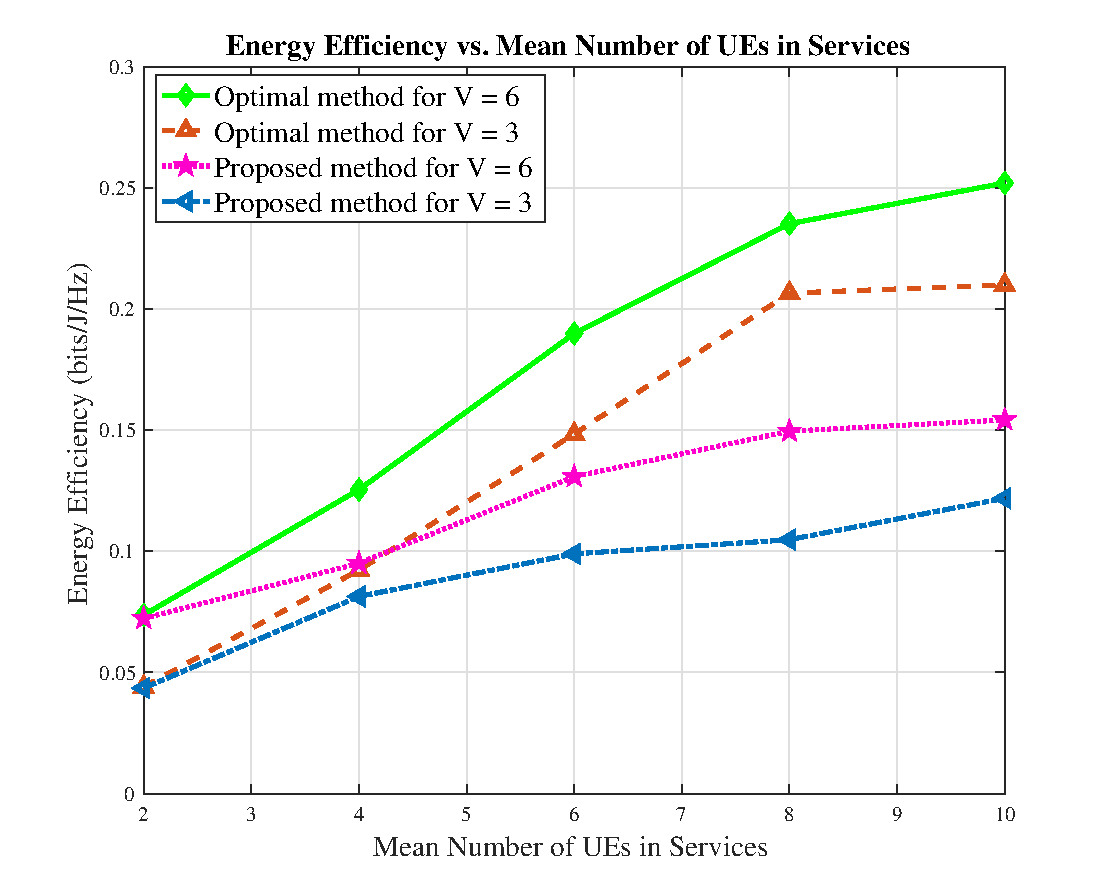
\includegraphics[width=\linewidth]{./fig/fig1_last}
	\caption{بهره‌وری انرژی براساس تعداد کاربران در هر سرویس}
	\label{fig:f1a}
\end{figure}
در شکل \ref{fig:f1a2}
بهره‌وری انرژی براساس تعداد بلوکهای منابع فیزیکی برای ۶ سرویس با تعداد کاربر به طور میانگین ۳ تا رسم شده است. همانطور که در نمودارها مشخص است با افزایش تعداد PRB، تداخل کاربران کم شده و بهره‌وری انرژی افزایش می‌یابد و الگوریتم پیشنهادی به روش بهینه نزدیک می‌گردد.  
\begin{figure}%[H]
	\centering
	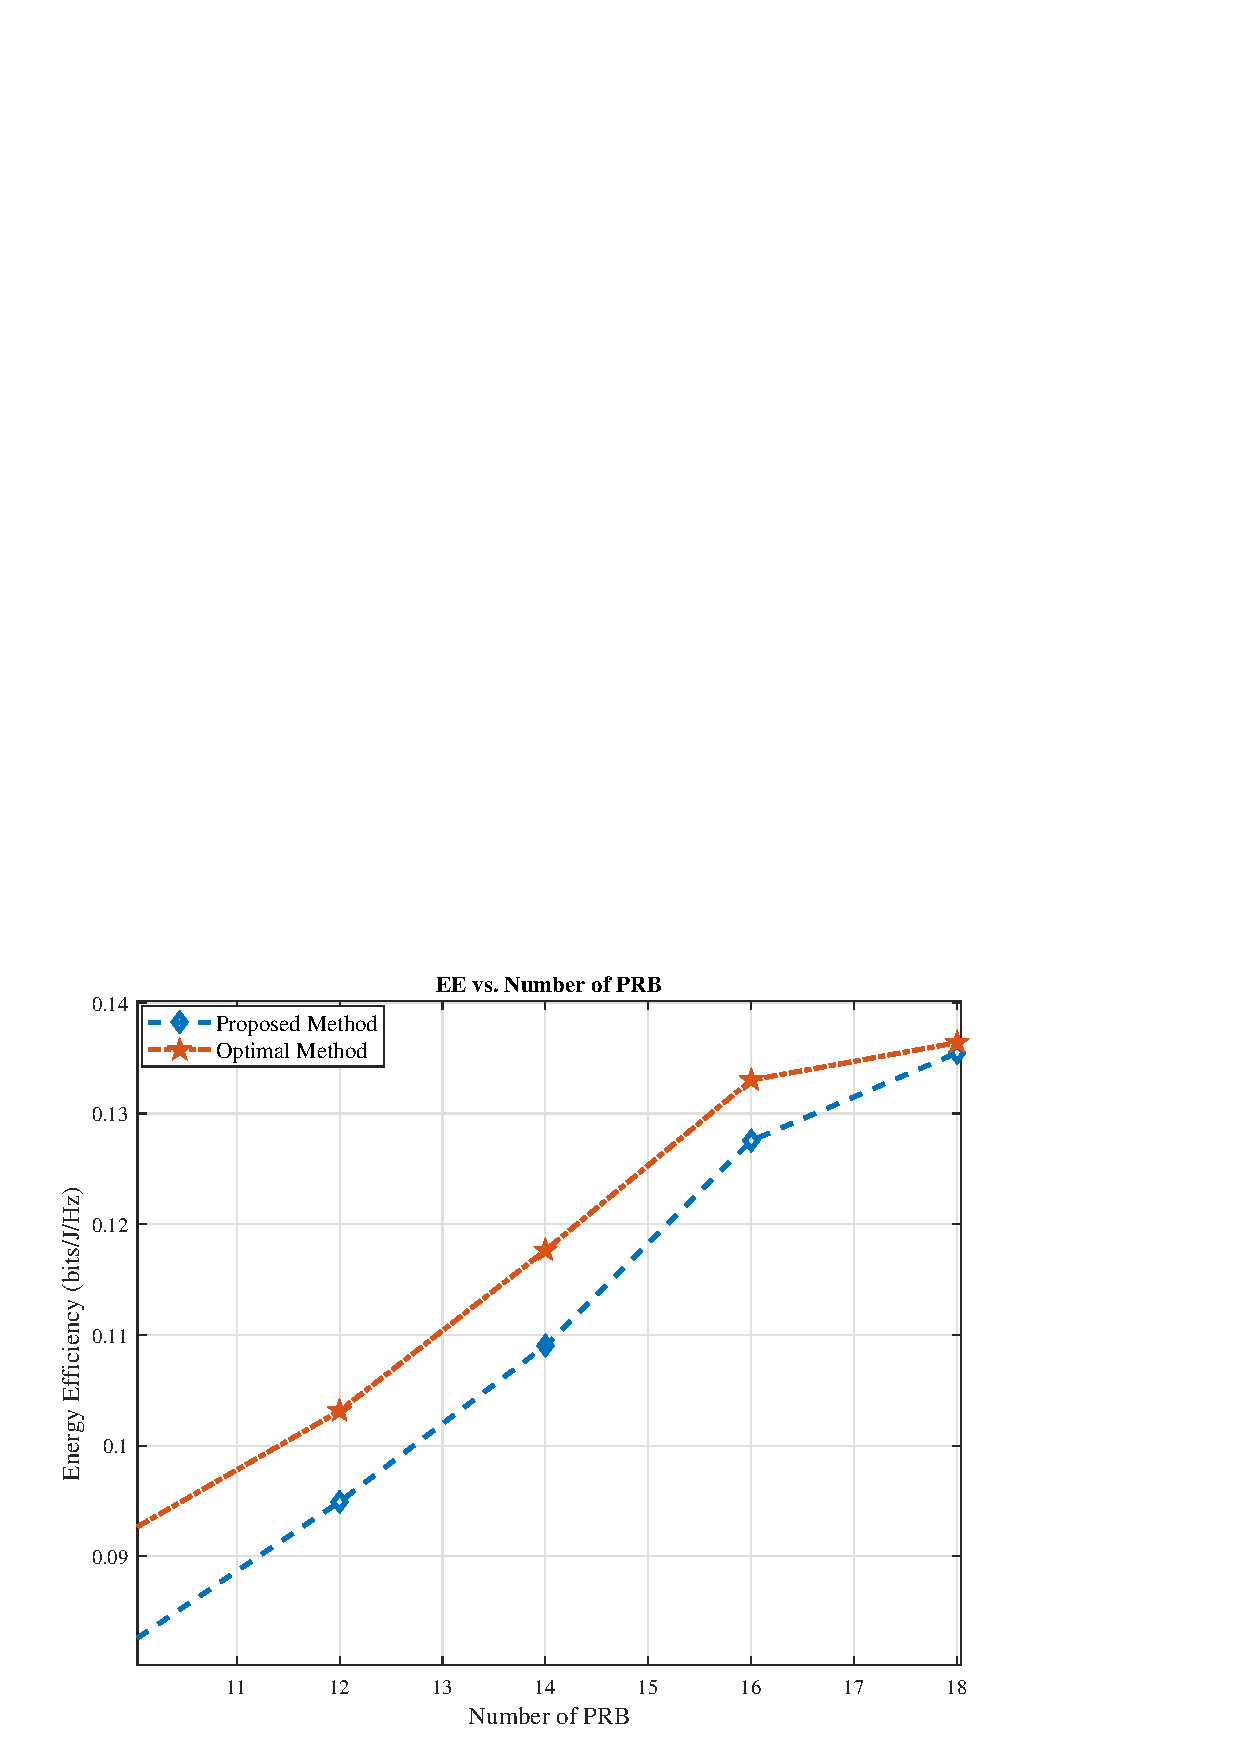
\includegraphics[width=\linewidth]{./fig/fig_prb}
	\caption{بهره‌وری انرژی براساس تعداد بلوکهای منابع فیزیکی}
	\label{fig:f1a2}
\end{figure}

در شکل \ref{fig:f1a3}
بهره‌وری انرژی براساس تعداد سرویسای مختلف با فرض وجود ۲ کاربر در هر سرویس به طور میانگین، رسم شده است. همانطور که در نمودارها مشخص است با افزایش تعداد سرویسها، بهره‌وری انرژی که مجموع نرخهای کاربران برروی توان آن است، افزایش می‌یابد و الگوریتم پیشنهادی به روش بهینه به نسبت نزدیک است‌.  
\begin{figure}%[H]
	\centering
	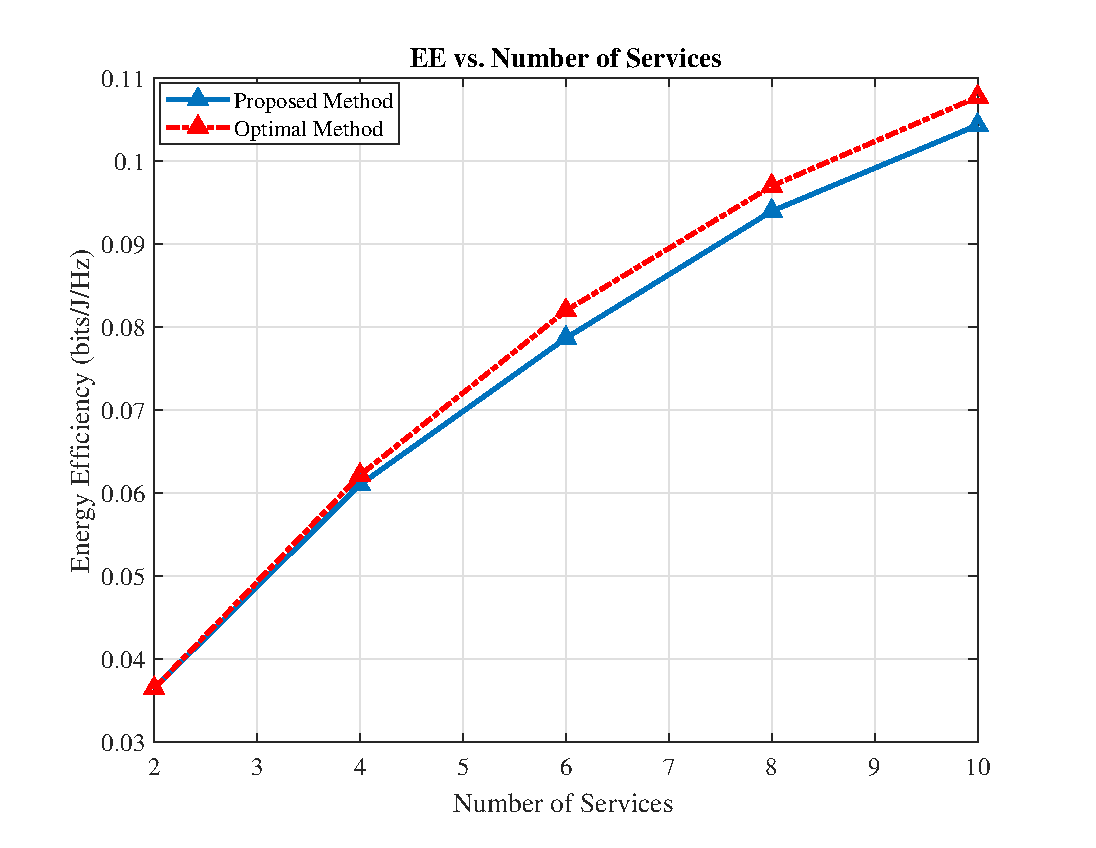
\includegraphics[width=\linewidth]{./fig/fig_service}
	\caption{بهره‌وری انرژی براساس تعداد سرویسهای مختلف }
	\label{fig:f1a3}
\end{figure}


حال به نتایج عددی مسئله‌ی دوم می‌پردازیم.
در شکل \ref{fig:f1}، نسبت برشهای پذیرفته شده برای دو تعداد مختلف مرکز داده با تعداد برشهای مختلف رسم شده است. پارامترهای شبیه‌سازی در جدول \ref{table:1} آورده شده است. همچنین داریم 
 $w_C = 320$،
 $w_S = 100$و 
 $w_M =1$.
 در این شبیه‌سازی ترم دوم رابطه‌ی \eqref{eqpsi}، مورد اهمیت قرار گرفته شده است و پارامتر طراحی $\nu$ مقدار بالایی دارد.
 همچنین فرض شده که تنها یک مرکز داده می‌تواند هر برش را سرویس دهد. روش ارائه شده در الگوریتم  \ref{alg3} آورده شده و روش بهینه با استفاده از MOSEK بدست می‌آید.
 وقتی دو مرکز داده یا DC داریم، روش پیشنهادی و روش بهینه تقریباً همان نسبت برش های پذیرفته شده را دارند. اما با افزایش تعداد DC ها به پنج ، عملکرد روش پیشنهادی کاهش می‌یابد.
 با استفاده از پنج DC ، تفاوت بین روش پیشنهادی و روش بهینه در بدترین حالت (44 برش) حدود 23 درصد است.

\begin{small}
	\begin{table}
		\caption {پارامترهای شبیه‌سازی} \label{table:1}
		\begin{latin}	
		\begin{center}
			\begin{tabular}{||c c ||}
				\hline
				Parameter & Value \\ [0.5ex]
				\hline\hline
				Mean of CPU for DCs & 320GHz\\
				\hline
				Mean of Memory for DCs & 1T\\
				\hline
				Mean of Storage for DCs & 100T \\
				\hline
				Mean of CPU for Slices & 32GHz\\
				\hline
				Mean of Memory for Slices & 100G\\
				\hline
				Mean of Storage for Slices & 10T \\ [1ex]
				\hline
			\end{tabular}
		\end{center}
	\end{latin}
	\end{table}
\end{small}
\begin{figure}%[H]
	\centering
	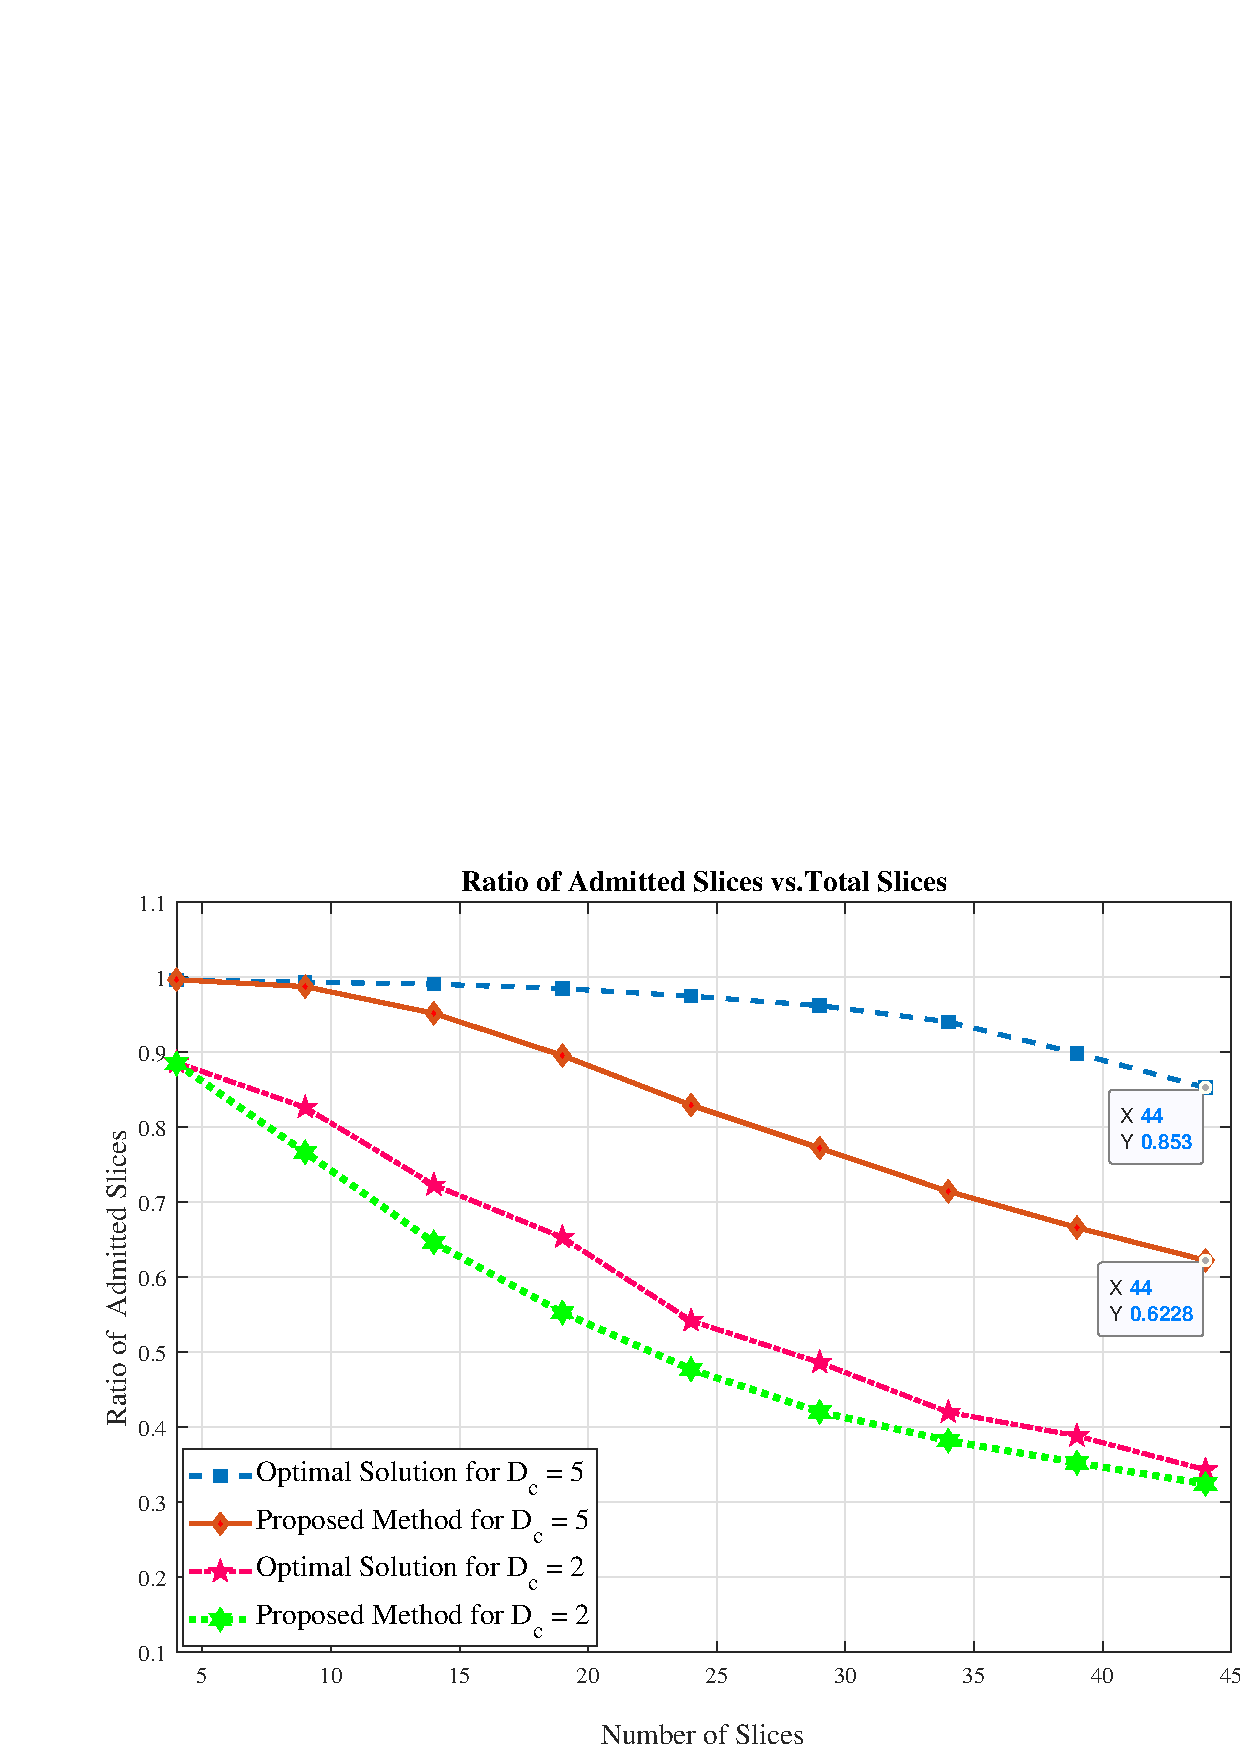
\includegraphics[scale = 0.5]{./fig/f112}
	\caption{نسبت برش های پذیرفته شده فقط به یک 	DC در مقابل برش های کل}
	\label{fig:f1}
\end{figure}
در شکل \ref{fig:f2}
نرمالیزه‌ی مصرف منابع بر‌اساس تعداد برشهای شبکه آورده شده است. پارامترهای شبیه‌سازی در جدول \ref{table:1}، قرار داده شده و 
($w_C = 320$, $w_S = 100$, $w_M =1$).
در این شبیه سازی ، فرض کنید تعداد DC ها کاملاً کافی باشد تا تمام برش ها را پوشش دهد و پارامتر طراحی شده $ \ nu $ کم فرض شود ، بنابراین ما روی اولین ترم \eqref{eqpsi} تمرکز کردیم.
با این حال ، اگر هر قطعه باقی مانده باشد ، می تواند توسط بیش از یک DC سرویس دهی شود.
بهینه بودن محل قرارگیری برشها در منابع DC بر اساس مصرف توان DC ها اندازه گیری می شود.
در اینجا مقدار منابع  مصرف DC نشده نشان داده شده است. برای ۱۰ برش شبکه اختلاف بین مقدار بهینه و روش اعمال شده ۱۵ درصد می‌باشد. 
\begin{figure}%[H]
	\centering
	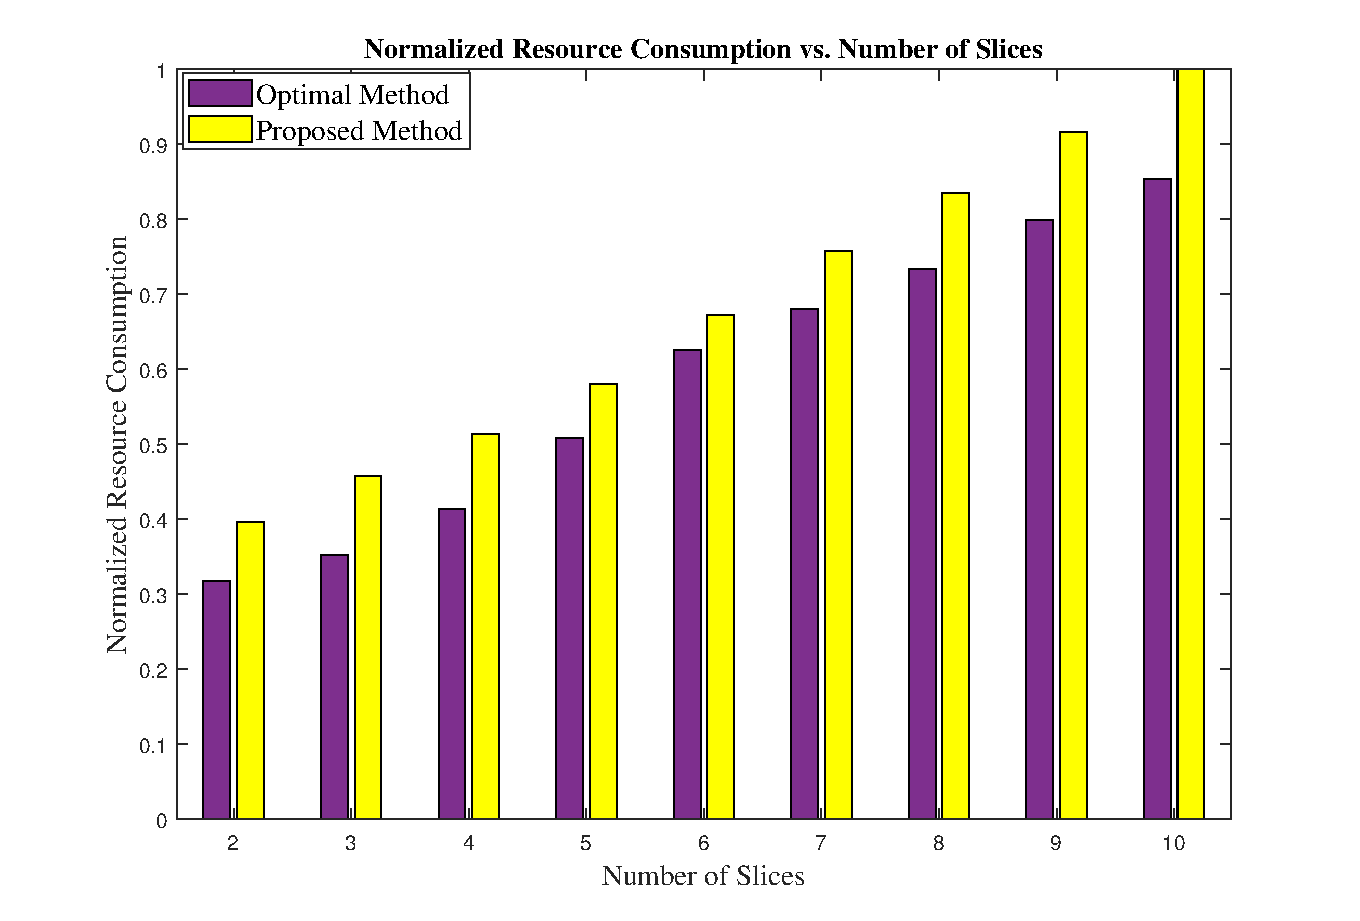
\includegraphics[scale = 0.5]{./fig/fig22_last} %[width=\linewidth] 
	\caption{نرمالیزه‌ی مصرف منابع بر‌اساس تعداد برشها}
	\label{fig:f2}
\end{figure}
\section{نتیجه‌گیری}
در این فصل، همزمانی برش شبکه و تخصیص توان در سیستم ORAN آمده‌است. فرض بر این است که کاربران بر اساس نیازهایشان به سرویسهای مختلف طبقه بندی می شوند. همچنین ، تعدادی برش نیز در خدمت این سرویسها قرار می‌گیرد. هر برش شبکه شامل تعدادی PRB، RU، و VNFهایی است که اعمال CU و DU را انجام می‌دهد. ظرفیت محدود لینک fronthaul برای اتصالات فیبر بین RU و DU در نظر گرفته شده است.
هدف به حداکثر رساندن مجموع نرخ و به حداقل رساندن مصرف توان و هزینه انرژی مراکز داده به طور همزمان است.
این مسئله به دو زیر مسئله تجزیه می شود. هر زیر مسئله به طور جداگانه توسط یک الگوریتم ابتکاری حل می شود. با استفاده از نتایج عددی، روش اکتشافی را تأیید کرده و عملکرد الگوریتم ها را مطالعه می کنیم.
برای مسئله‌ی اول بازدهی انرژی در مقابل تعداد UE در هر سرویس به تصویر کشیده شده است.
با افزایش میانگین تعداد کاربران در هر سرویس، از بازدهی انرژی بیشتر می‌شود.
برای مسئله دو، دو شکل نشان داده شده است.
در شکل اول، نسبت برش های پذیرفته شده که فقط به یک DC متصل می‌شوند، برای تعداد برش های مختلف مشخص شده است.
در شکل دوم ، مصرف منابع نرمال DC ها به تصویر کشیده شده است.
در هر شکل ، الگوریتم ابتکاری با روش بهینه مقایسه شده و تفاوت بین آنها بحث شده است.

